\begin{figure}[htbp]
\centering
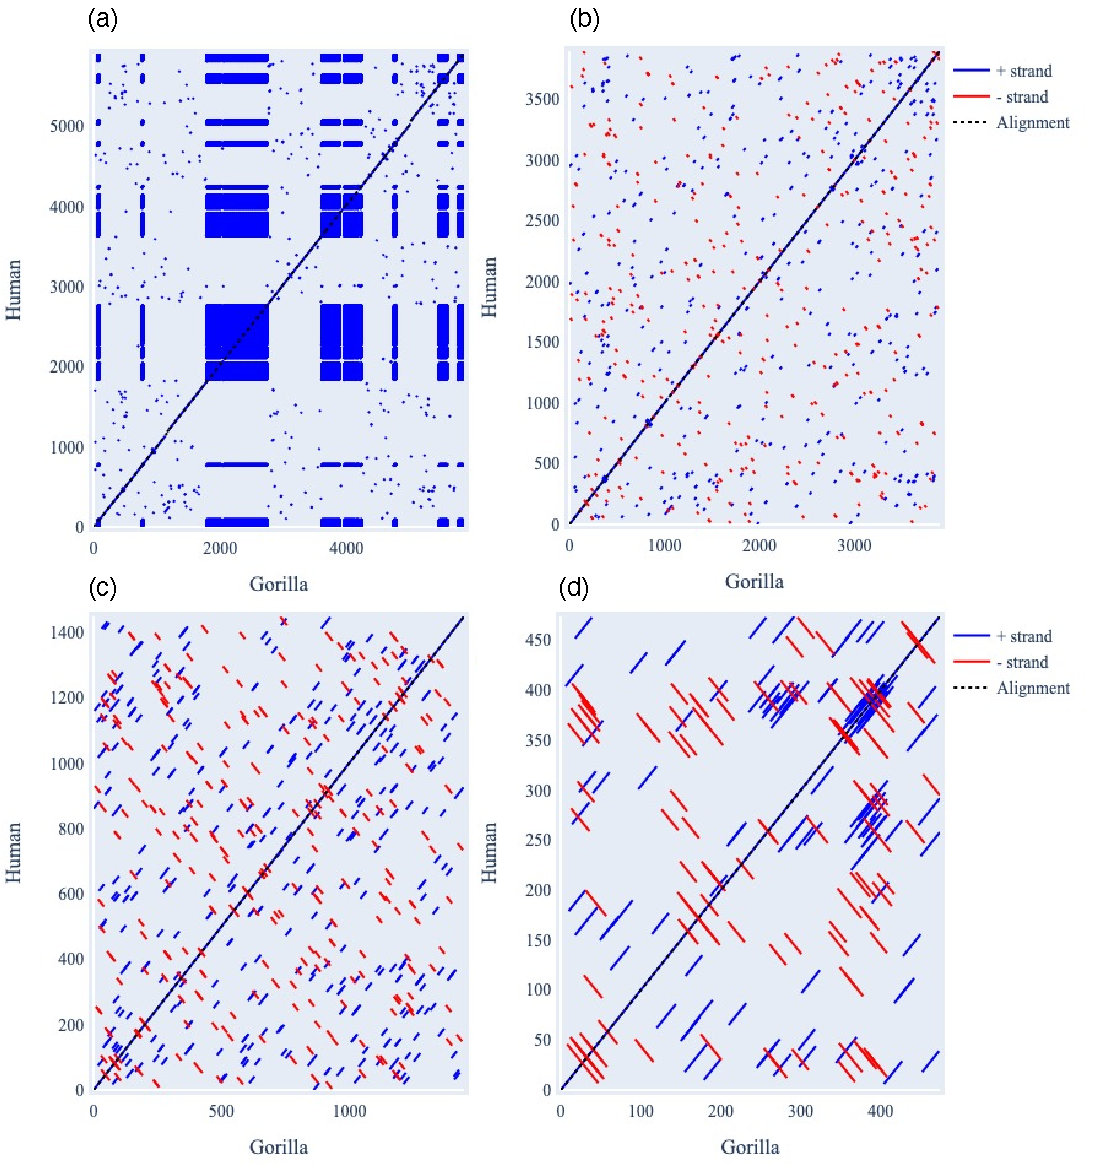
\includegraphics[width=\textwidth]{figures/diagrams/primate_dotplots.pdf}
\caption[Dotplots of an intronic and CDS alignment before and after filtering]{\textbf{Dotplots of an intronic and CDS alignment before and after filtering}. \textbf{(a)}, intronic pre-filtering, \textbf{(b)} intronic post-filtering, \textbf{(c)} CDS pre-filtering, \textbf{(d)}, CDS post-filtering. The alignment path between the sequences is shown as the dotted line. Long stretches of identity between sequences form a diagonal. Long stretches of tandem repeats show up as large blocks of colour, visible in (a). The window was 20bp long, 20-mers identical at $>13$ positions were considered a match. The $x$- and $y$-axis are positions in the unaligned sequence. The Ensembl unique identifiers for the chosen intron and CDS alignment were ENSG00000181036 and ENSG00000116704 respectively.}
\label{fig:dotplots}
\end{figure}